\begin{block}{\texttt{QSplit} Results}
    We tested \texttt{QSplit} with problems from 128 variables, and the data collected showed the following behaviour \textbf{when decreasing the Stopping dimension}.

    \begin{figure}[h!]
        \centering
        \begin{minipage}{0.55\textwidth}
            \centering
            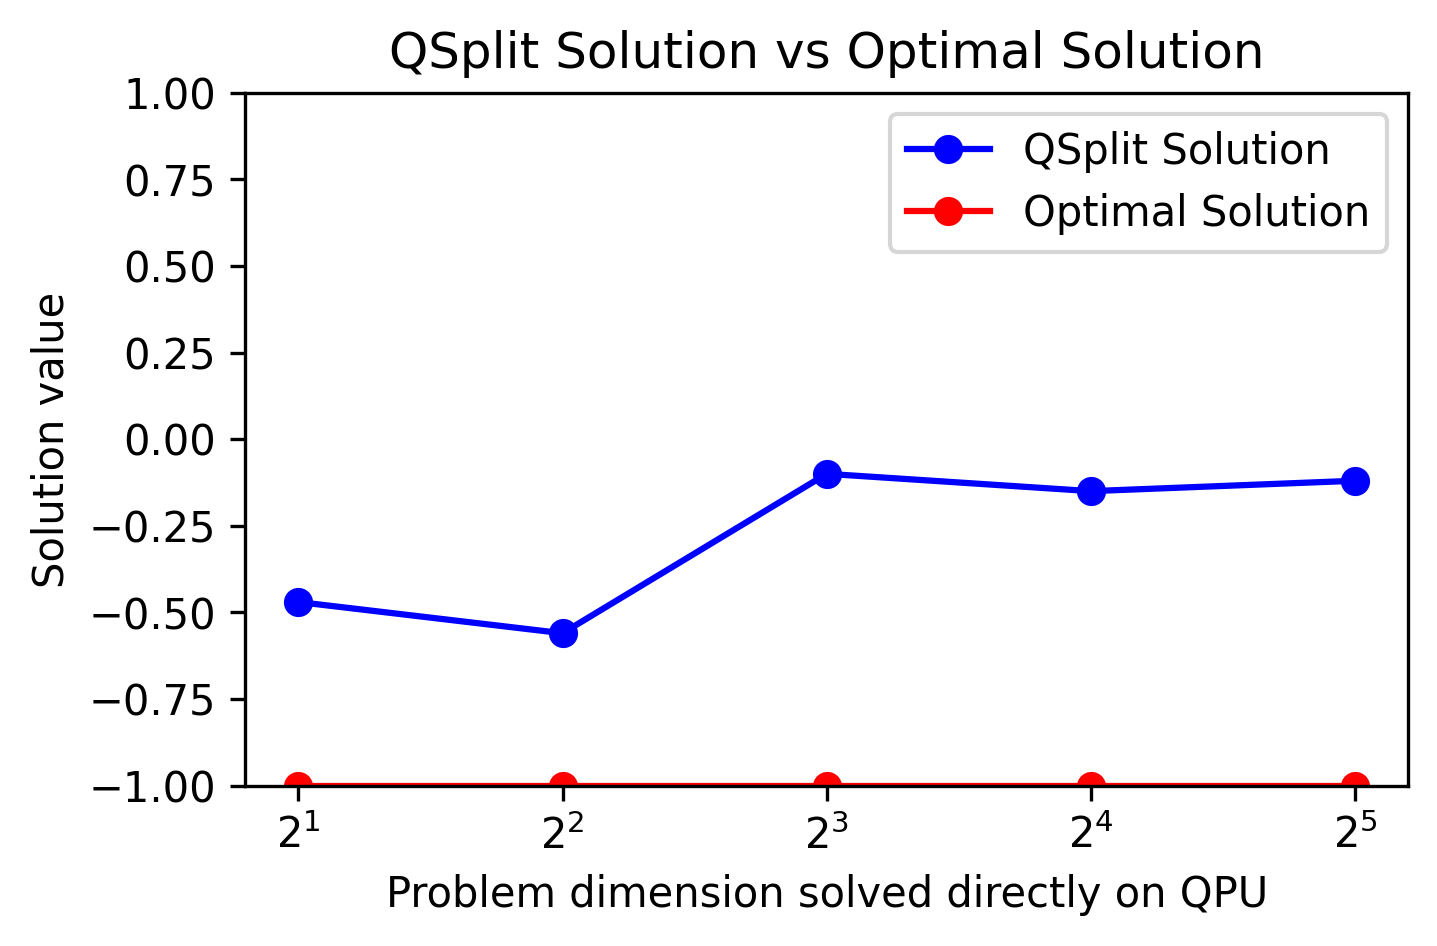
\includegraphics[height=0.14\textheight]{logos/sol.png}
        \end{minipage}%
        \hfill
        \begin{minipage}{0.4\textwidth}
            \begin{alertblock}{Performance}
                The quality of the solution improves, with the error decreasing from 45\% to 25\%.
            \end{alertblock}
        \end{minipage}
    \end{figure}

    \begin{figure}[h!]
        \centering
        \begin{minipage}{0.4\textwidth}
            \begin{alertblock}{Execution Time}
                The time required by \texttt{QSplit} increases, ranging from requiring 40\% less time compared to direct resolution to requiring 50\% more time.
            \end{alertblock}
        \end{minipage}%
        \hfill
        \begin{minipage}{0.55\textwidth}
            \centering
            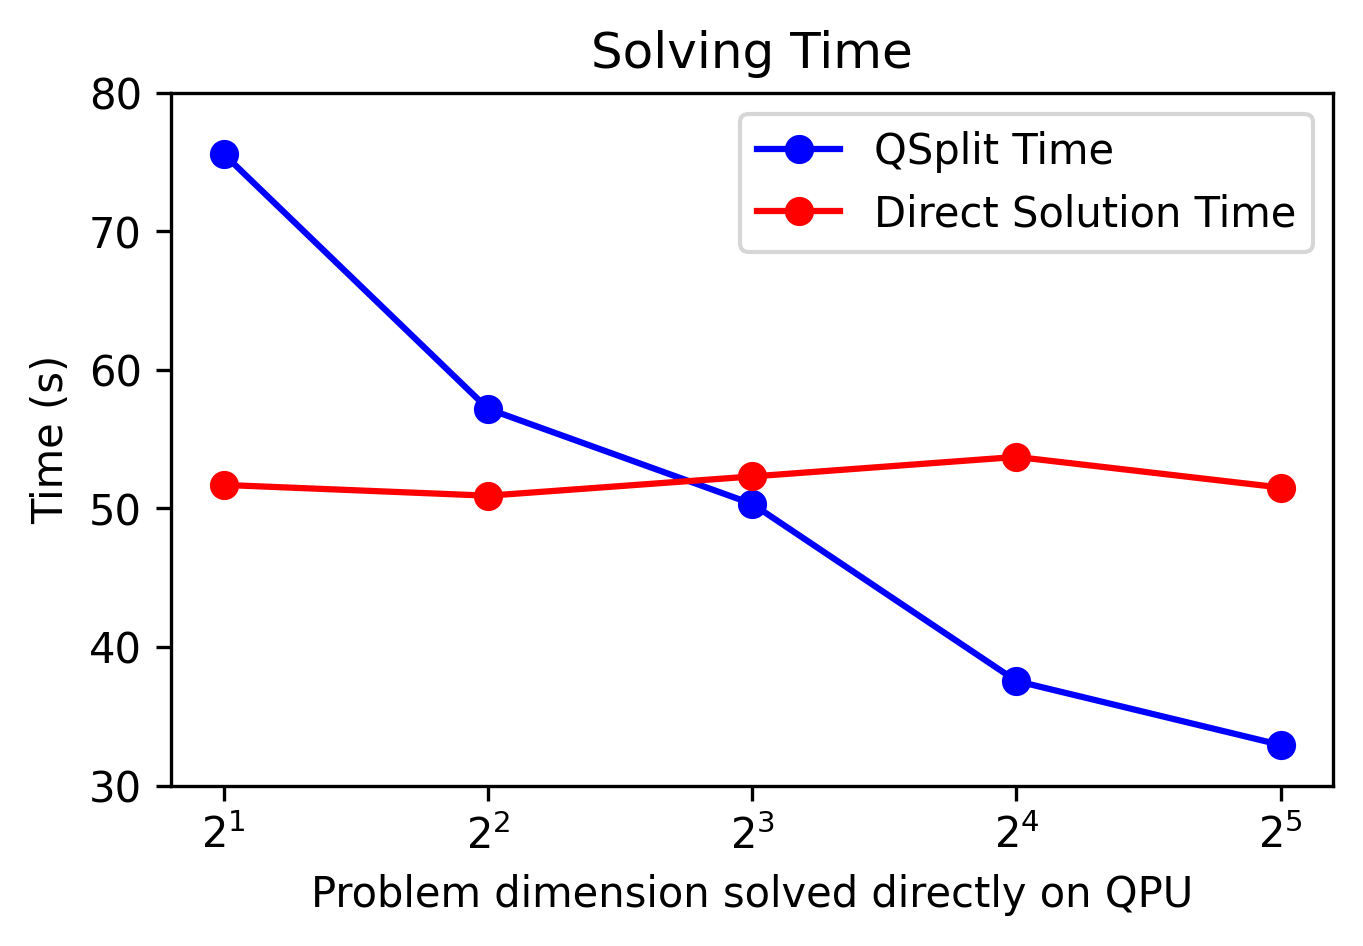
\includegraphics[height=0.14\textheight]{logos/time.png}
        \end{minipage}
    \end{figure}
\end{block}